\documentclass[minted, en]{thesis}
\usepackage{parskip}
\usepackage{textcomp}
\usepackage{tablefootnote}
\usepackage{appendix}
%Advanced Hyphonation
\usepackage{microtype}

% Required
\title{Plant Whispers}
% Authors
\author{Simon Puschmann}{5AHIT}{Elektronik Sensor und Messtechnik}
\author{Jacob Szücs}{5AHIT}{Filtern und vorbereiten der Daten}
\author{Fabian Geiblinger}{5AHIT}{Speichern und Zuweisen der Daten}
\author{Simon Wewalka}{5AHIT}{Auswerden der Daten}
\author{Julian Kropatschek}{5AHIT}{Benutzeroberfläche}
% Date of submission
\date{4. April 2023}
% Optional
\mysubtitle{}
\myteacher{Dipl. Ing. Roland Strohmer}
\myyear{2023/24}
\mydivision{Systemtechnik}
\selectlanguage{english}			% Set language to english
% \selectlanguage{ngerman}			% Set language to german
% \setcode{frame=single} 			% Add a frame to codes
% \setcode{bgcolor=AlmostWhite}		% Add a background to codes (minted only)
% \usemintedstyle{rainbow_dash} 	% autumn, rainbow_dash, tango (default), trac
\begin{document}
%!TEX root=../main.tex

% German abstract
\begin{abstract}[ngerman]
Im Rahmen des vorliegenden Projekts soll in Kollaboration mit der Plants Facility des Vienna-BioCenters ein neuartiges Werkzeug zur weiteren Erforschung von Pflanzenstress entwickelt werden. Eine kürzlich von Cell veröffentlichte Studie hat gezeigt, dass bestimmte Pflanzen unter Stress hochfrequente Klickgeräusche erzeugen können. Dieses Phänomen bildet die Grundlage für diese Diplomarbeit. Viele Bioakustikforschungsteams forschen aktuell an diesem Phänomen was diese Arbeit hochaktuell und relevant für unseren Projektpartner macht.

\end{abstract}

% English abstract
\begin{abstract}[english]

In this project, a tool for further research on plant stress will be developed in collaboration with the Plants Facility of the Vienna-BioCenter. A recent study published by Cell has shown that certain plants can produce high frequency clicking sounds under stress. This phenomenon forms the basis for our work. Many bioacoustics research teams are currently researching this phenomenon which makes this work highly relevant.

\end{abstract}
% Table of contents
\tableofcontents\glsresetall
\newpage\pagestyle{fancy}

%!TEX root=../main.tex
\chapter{Danksagung} 

In erster Linie wollen wir uns als Projektteam bei unseren Projektbetreuern bedanken. 

Danke an \textbf{Salvatore Trautenberg}, für UZZUZZ als Ausgleich zur harten arbeit
%!TEX root=../main.tex
\chapter{Vorwort}
Die Diplomarbeit ist kein Aufsatz!
Auch wenn sie interessant gestaltet werden sollte, ist sie unpersönlich und im passiv zu schreiben.
Besonders sind die Quellenangaben, welche entsprechend gewählt und referenziert werden müssen.
Innerhalb dieser Vorlage existieren 2 Dateien, die zu genau diesem Zweck erstellt wurden. Die Datei \verb|bibliography.bib| beinhaltet alle Quellenangaben und verwendete Literatur, \verb|glossaries.tex| alle Definitionen von Begriffen und Akronymen, welche in der Arbeit selbst nicht genauer erklärt werden.
 			% Include the chapter „Vorwort“
%!TEX root=../../main.tex
\section{Quellen} 
Das richtige zitieren spielt innerhalb der wissenschaftlichen Arbeit eine wichtige Rolle. Die Vorlage nutzt zur Verwaltung von Literatur ein Programm mit dem Namen \verb|biblatex|. Mit diesem werden alle Einträge, welche sich in der Datei \verb|bibliography.bib| befinden verarbeitet und können in der Arbeit selbst über das Kommando \codeinline{latex}{\cite{key}} referenziert werden.

Als kleines Beispiel findet sich hier nun ein Zitat über Schall, aus dem ersten Phsyik Lehrbuch der Autoren, Schweitzer, Svoboda und Trieb.

\begin{quote}
\enquote{Mechanische Longitudinalwellen werden als Schall bezeichnet. In einem Frequenzbereich von 16 Hz bis 20 kHz sind sie für das menschliche Ohr wahrnehmbar. Liegen die Frequenzen unter diesem Bereich, so bezeichnet man diese Wellen als Infraschall, darüber als Ultraschall.} \cite[S. 145]{physik1}
\end{quote}

Eine Referenz wie diese ist möglich, wenn der entsprechende Eintrag in der dafür vorgesehenen Datei vorhanden ist. In diesem Fall sieht die Definition der Quelle wie folgt aus:

\begin{listing}
\begin{code}{bibtex}
@book{ physik1,
	title = {Physik 1},
	author = {Christian Schweitzer, Peter Svoboda, Lutz Trieb},
	year = {2011},
	subtitle = {Mechanik, Thermodynamik, Optik},
	edition = {7. Auflage},
	publisher = {Veritas},
	pages = {140, 145-150},
	pagetotal = {296}
}
\end{code}
\caption{Eintrag einer Buchquelle in BibLatex}
\end{listing}

Bei einem direkten Zitat empfiehlt es sich auch die Seitenzahl anzugeben. Dies kann über die Option des Kommandos \codeinline{latex}{\code[S. Zahl]{key}} bewerkstelligt werden.
    
Nach der Verwendung einer Quelle, wird diese auch im Literaturverzeichnis gelistet, welche sich am Ende des Dokuments befindet.	% Include a section of a chapter
%!TEX root=../main.tex
\chapter{Einleitung} 

\section{Gender Erklärung}
Aus Gründen der besseren Inklusion wird diese Diplomarbeit geschlechtsneutral verfasst.
Diese Entscheidung wurde in Absprache mit allen Projektmitgliedern getroffen, da die Inklusion ein Aspekt ist, auf den großen Wert gelegt wird.

\section{Was ist PlantWhispers}
Die Vorliegende Diplomarbeit beschreibt eine weitestgehend automatisierte Lösung zur Forschung an Pflanzen-Akustik. Das Projekt beschäftigt sich mit dem Prozess von der Messung bis hin zur Bereitstellung der Daten, und soll Forschenden Repetitive Arbeit abnehmen.

\section{Zielsetzung}
Um in der Forschung von möglichst großem Nutzen zu sein, muss die Bedienung des Systems ohne hoher IT Expertise möglich sein. Sowohl Rohdaten, als auch anschauliche Graphen werden den Benutzenden zur Verfügung gestellt.

\section{Nutzen}
Pflanzen-Akustik ist ein weitaus unerkundetes Forschungsgebiet. Laut einer im Frühjahr 2023 veröffentlichten Studie \cite{Cell_Sounds_emitted_by_plants} kann durch die Aufnahme von Pflanzen-Geräusche in einer Gewächshaus-Umgebungen wertvolle Informationen über den Stress der Pflanze herausgefunden werden.

%Zu Beginn wird die Ausgangslage beschrieben, wobei interessant ist woher das Projekt kommt und welche Ansätze an dessen Konzept beteiligt waren. Hier werden auch Ziele gesetzt und Probleme bestimmt, welche in der Arbeit selbst eine große Rolle spielen.Expertise

%Im Rahmen des vorliegenden Projekts wird in Kollaboration mit der Plants Facility des Vienna-BioCenters ein neuartiges Werkzeug zur weiteren Erforschung von Pflanzenstress entwickelt. Eine kürzlich von Cell veröffentlichte Studie hat gezeigt, dass bestimmte Pflanzen unter Stress hochfrequente Klickgeräusche erzeugen können. Dieses Phänomen bildet die Grundlage für diese Diplomarbeit. Eine bedeutende Motivation für die Ausarbeitung von diesem Projekt besteht darin, dass es von Grund auf verschiedene technische Methodiken miteinander verknüpft. Dadurch eröffnet sich die Möglichkeit, eine breite Vielfalt an Fähigkeiten und Wissen zu erwerben, was diese Arbeit zu einer besonders herausfordernden und lehrreichen Erfahrung macht.


%STUDIE
%!TEX root=../main.tex
\chapter{Studie}
Nach der Definition der Problemstellungen und Ziel soll recherchiert werden, wie diese erreicht, beziehungsweise gelöst werden können. Diese Studie beschäftigt sich mit möglichen Lösungen und Technologien und analysiert deren Eigenschaften um konkrete Vor- und Nachteile zu finden.
Beendet wird dieser Abschnitt mit einem Fazit.

\section{Fazit}
Das Fazit soll zeigen, wie das Projekt durchgeführt werden kann.


\include{chapters/Studie/Phänotyp}
\section{Pflanzenstress}
Unter dem Begriff Pflanzenstress versteht man es in der Biologie,dass Pflanzen verschiedenen Faktoren ausgesetzt werden, welche unnatürlich oder kritisch für eine Pflanze sind und somit in dieser Pflanze dann die Freisetzung von verschiedenen Terpenen, Fettsäurederivaten, Benzoiden, Phenylpropanoiden und von Aminosäuren abgeleiteten Stoffwechselprodukten auslösen. \cite{jk2010multiple}

\subsection{verschiedene Auslöser von Pflanzenstress}
Bei allen hier aufgelisteten Auslösern ist zu beachten, dass verschiedene Pflanzengattungen unterschiedlichst auf die folgenden Faktoren reagieren und andere Schwellenwerte haben. Alle diese Stressfaktoren können auch irreparable Schäden an Pflanzen anrichten.
Man kann die Stressfaktoren in drei große Gruppen unterteilen\cite{gaspar2002concepts}:
\begin{itemize}
  \item physiche Faktoren
  \item chemische Faktoren
  \item biotische Faktoren
\end{itemize}

\subsubsection{physiche Stressfaktoren}


\paragraph{Wasserstress} ist ein klassischer physischer Stressfaktor. Unter Wasserstress versteht man es, eine Pflanze einer ungeeigneten Menge an Wasser auszusetzen. Dies bedeuted in der Praxis meist, dass man die Pflanze unterbewässert. Theoretisch kann man natürlich auch die Pflanze überbewässern, was weniger oft Einsatz in der Forschung findet.

\paragraph{Temperaturstress} bedeuted, eine Pflanze durch entweder Kälte- oder Wärmestress zu beinflussen.
Kalte Temperaturen  können die Aufnahme von Wasser und Nährstoffen beeinträchtigen. Dies kann zum Austrocknen(Trockenstress) und Verhungern der Zellen führen. Bei extrem kalten Bedingungen kann die Zellflüssigkeit gefrieren, was zum Tod der Pflanze führt. Zu hohe Temperaturen haben auch negativen Einfluss. Durch zu hohe Temperaturen können Zellproteine abgebaut werden oder Zellwände und -membrane können Schmelzen. Temperaturschwankungen führen also zu Stress und Beinträchtigung der normalen Funktionen einer Pflanze. Auch Temperaturstress ist ein klassischer physischer Faktor.


\paragraph{Strahlung, Wind} und weitere Faktoren können auch natürlich auftreten werden aber in dieser Arbeit keine Verwendung finden 

\subsubsection{chemische Stressfaktoren}

\paragraph{Toxine} kommen in der Natur und in der Agrarwelt oft vor. Diese können zum Beispiel über verschmutztes Grundwasser aufgenommen werden und die natürliche Funktion einer Pflanze stark einschränken. Oft werden Toxine auch in Form von Luftverschmutzung von Pflanzen aufgenommen.

\paragraph{Pestizide und Fungizide} finden oft in der Landwirtschaft Einsatz. Gerade deshalb sollte nicht vergessen werden, dass auch diese starken chemischen Stress auslösen können.

\subsubsection{Biotische Stressfaktoren}

\paragraph{Krankheiten, Pilze und Viren} sind die am häufigsten autretenden boitischen Stressfaktoren indem diese eine Pflanze befallen und diese schwächen.

% METHODIK

\subsection{Methodik zur Erfassung des Pflanzenstresses}

Pflanzenstress wird schon länger erforscht, wobei sich die meisten Messmethodiken auf Bilderkennung, Thermalbilder, 3D Scans und auf Hyperspektralbilder zurückgreifen. Es gibt auch weitere Möglichkeiten den Pflanzenstress zu erkennen, jedoch sind das die aktuell am häufigsten verwendeten in der Pflanzenpathologie.
\cite{behmann2015detektion}\cite{messtechniken}

\subsubsection{RGB Bildanalyse}
Durch eine digitale RGB-Farbbildgebung in Verbindung mit einer automatischen, analytischen Software ist eine Extraktion von verschiedenen Merkmalen möglich. Hochauflösende kinetische Messungen werden für eine eingehende Analyse der Pflanzenmorphologie, Architektur und zur Extraktion von Farbindexmerkmalen verwendet.

\subsubsection{3D-Laserscans}
 Ein Laserstrahl wird von der Pflanze reflektiert und von einer Kamera erfasst. Ein automatisierter Phänotypisierungsprozess beinhaltet also das Scannen der Pflanze, die Erstellung eines 3D-Modells, die Erhebung von Pflanzenparametern und die anschließende Analyse. Auf der Grundlage der vernetzten Modelle bietet die automatische Datenanalyse die Berechnung einer breiten Palette von morphologischen Parametern.\cite{vandenberghe2018make}

Diese Technologien und Verfahren ermöglichen eine detaillierte Erfassung und Analyse der Pflanzenmorphologie und -struktur, was für die Erforschung von Pflanzenreaktionen auf verschiedene Stressbedingungen wichtig ist.

\subsubsection{PAM chlorophyll fluorescence}
Die Chlorophyllfluoreszenz-Analyse, insbesondere mittels Puls-Amplituden-Modulation (PAM), ist eine bewährte Methode zur Beurteilung der Photosyntheseleistung und des physiologischen Zustands von Pflanzen, einschließlich des Stresses, dem sie ausgesetzt sind.

Zuerst wirden die Chlorophyllmoleküle in den Pflanzenzellen mittels Lichtmolekülen angeregt. Im angerregten Zustand emittieren die Chlorophyllmoleküle Licht. Die Intensität dieses Lichtes kann dann gemessen und verarbeitet werden.
Änderungen in den Fluoreszenzparametern können auf Stressbedingungen hindeuten, unter denen die Pflanze steht.

Diese Methode ist nicht-invasiv und ermöglicht eine schnelle und genaue Einschätzung des physiologischen Zustands von Pflanzen, was sie zu einem wertvollen Werkzeug für die Pflanzenphänotypisierung und die Bewertung von Pflanzenstress macht.

\subsubsection{LWIR thermal imaging}

\subsubsection{Hyperspectral imaging (VNIR and SVIR)}

\section{PHENOBox}
As part of our collaboration with the Vienna Bio Center, we were provided with the so-called PHENOBox as a product environment. The PHENOBox is a flexible solution for plant phenotyping research using image data. During the course of our diploma project, the PHENOBox will be equipped with 2 high-frequency microphones. \cite{czedik-eysenberg_phenobox_2018}

\subsection{Technical Specifications}
The PHENOBox has a height of 75.5 cm, a width of 50 cm, and a length of 82 cm (side) + 4 cm (door handle). It weighs approximately 15 kg. The imaging area is suitable for plants with a maximum shoot size of about 20 cm in width and 40 cm in height. \cite{czedik-eysenberg_phenobox_2018}

The camera can be adjusted in height to achieve a centered position on the shoot for imaging. A Canon SLR camera (700D) is installed in the PHENOBox for easy operation and high image quality. \cite{czedik-eysenberg_phenobox_2018}

The homogeneous illumination of the imaging area is achieved by 7 LED panels, two on each side of the image axis (vertical) and three (horizontal) above the shoot imaging area. \cite{czedik-eysenberg_phenobox_2018}

\section{PHENOPipe}
PhenoPipe is an open-source analysis platform for managing and evaluating samples that complements the hardware of the PhenoBox. It allows for the automation of image processing and data analysis and provides a web interface for managing phenotyping projects. The entire code for PHENOBox and PHENOPipe is located in a public Github repository. \cite{czedik-eysenberg_phenobox_2018}

\textbf{The code consists of the following components:}

\subsection{Phenobox}
Code for the Phenobox itself, which runs on a Raspberry Pi 3.\newline
Captures images and interacts with the Phenopipe server.

\subsection{PhenoPipe Web}
Main server with database and web interface.\newline
Written in Python with Flask and TypeScript with Angular.\newline
Manages experiments, labels, analyses, etc.

\subsection{PhenoPipe Postprocess Server}
A Java-GRPC server for postprocessing analysis data with R scripts.\newline
Setup instructions

\subsection{Phenopipe IAP Server}
A Java-GRPC server for interacting with the IAP (Image Analysis Pipeline).

Although the PHENOPipe has many features that could be potentially useful for our project the complexity and the lack of maintenance could bring more disadvantages than benefits.

\section{Analyzing and evaluating the data}

New, sophisticated techniques for categorizing ultrasonic sounds made by distressed plants now offer fresh approaches to non-invasive plant health monitoring and comprehension. The chapter critically examines the state-of-the-art methods used for classifying the stresslevel and/or stress-type of plants through such sounds and focuses on Support Vector Machines (SVM) and Convolutional Neural Networks (CNN). Due to the limited resources in the research of sounds emitted by plants this section is heavily dependent on the paper ``Sounds emitted by plants under stress are airborne and informative" \cite{Cell_Sounds_emitted_by_plants} published by Cell.








\subsection{Classifying plant sounds}
\subsubsection{Convolutional Neural Networks (CNN's)}
Convolutional Neural Networks (CNNs) form the base for deep learning in computer vision and, as such, the field of machine learning. CNNs can process grid-like data, and no technique can process images better than CNNs. They have shown efficiency in dealing with imagery that is visual because they make use of a model in a very hierarchical manner, which processes the data in consecutive layers of processing. These networks use convolutional layers, pooling layers, and fully connected layers in the feature extraction process thus making them highly effective for tasks such as image and sound classification.\cite{oshea_introduction_2015}

This type of architecture learns automatic and adaptive spatial hierarchies of features from the input. The convolutional layer applies some learnable filters on the input in order to extract spatial features like edges and textures. Every filter is small spatially but runs through the full depth of the input volume. This way, the network is able to detect features at different locations in the input. The pooling (or subsampling) layer then reduces the spatial size of the representation by down-sampling, and that aids in controlling the overfitting problem because the number of parameters and calculations in the network is reduced. \cite{oshea_introduction_2015}

CNNs have been proven to be very good for tasks related to sound classification owing to their excellent exploitation of the invariance property of the input. This is because the fact that CNNs are capable of learning and picking up the spectro-temporal patterns present in the data that distinguish different types of sounds. When applied to sound data, which is commonly in a spectrogram representation, this can be manifested by being able to identify different patterns related to a difference in sound or soundscape. \cite{salamon_deep_2017, piczak_environmental_2015}

Some of the studies have shown the potential of CNNs in sound classification and therefore indicate the possible breakthrough in detection and classification of environmental sounds from different datasets. Such sounds include urban noise, natural soundscapes, and man-made, among others. It clearly states that the performance of CNNs can be significantly enhanced in sound classification tasks by applying techniques like data augmentation that artificially enhances the diversity of the training set through time stretching, pitch shifting, and adding background noise transformations. These regularization approaches have been shown to improve the robustness of the model, hence also translating into better generalization capability and better performance on unseen data. \cite{salamon_deep_2017, piczak_environmental_2015}

Convolutional Neural Networks were used for classifying the sounds emitted by stressed plants, such as greenhouse noises and drought-stressed tomato sounds. The Python 3.6 programming language was used to build these models using Keras library with the tensorflow backend. In its design, there are three blocks where each of them contains two 1D convolution layers with ‘relu’ activation followed by a max pooling layer and a dropout layer which ended up with a fully connected layer with ‘relu’ activation and another dropout layer. The final layer for binary classification has sigmoid activation function meanwhile for multi-class classification (three categories), softmax activation is used. \cite{Cell_Sounds_emitted_by_plants}

\subsubsection{Support Vector Machines (SVM's)}
Support vector machines (SVMs) are a supervised learning method that can be used for classification, regression, and outliers detection. They have been most popularly used to classify two-group data sets. The classifier is developed by Vapnik in the 1990s based on the concept of decision planes that define decision boundaries. A decision plane is one that separates between a set of objects having different class memberships.

The SVM works by finding the hyperplane which best divides a dataset into two classes. Support vectors are the data points nearest to the hyperplane. The distance between the hyperplane and these support vectors constitutes as margin. The further apart these support vectors are from each other, and from the margin, the more accurate your classifier will be.

\begin{figure}
    \centering
    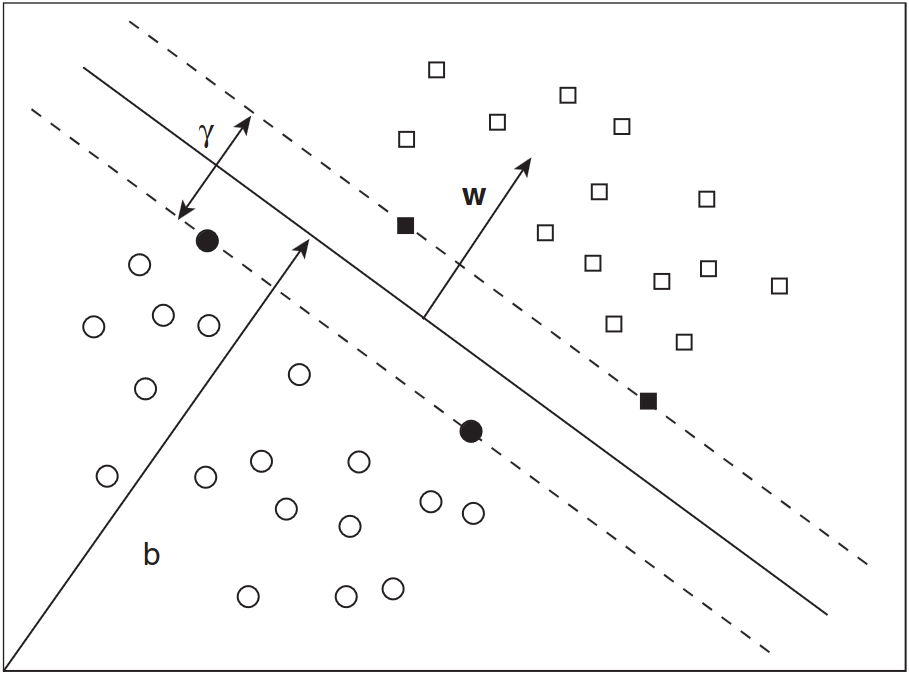
\includegraphics[width=0.5\linewidth]{images/svm.png}
    \caption{from ``Support vector machines" by Mammone\cite{mammone_support_2009}, A graphical rendering that outlines the steps taken in SVM linear classification in a two-dimensional feature space. In this model, circles and squares depict data points from two separate classifications. The solid line represents the hyperplane that was identified as the decision boundary by the SVM algorithm. Dotted lines are margins, and filled shapes (circles and squares) act as support vectors. Vector \textbf{w} is perpendicular to the hyperplane with a positive direction, while parameter \textbf{b} indicates how far off the origin the hyperplane lies. \textbf{y} is distance across each margin, which gets maxed out in SVM.}
    \label{fig:enter-label}
\end{figure}

Kernels are functions used in SVMs to transform your input data into a higher-dimensional space where it can then be separated more clearly with a hyperplane. This is particularly useful when you have non-linear separable problems. By mapping your low-dimensional feature space onto high-dimensional space, you're able to perform linear separation of data that is non-linearly separable in its original input space. \cite{mammone_support_2009}

When it comes to sound classification, SVMs could be used for differentiating between different types of sounds or determining characteristics of a single sound source. Support Vector Machines, in conjunction with a variety of feature extraction techniques, were utilized by the researchers to classify the types of stress experienced by plants, such as drought or physical damage like cuts. This involved basic features, Mel-frequency cepstral coefficients (MFCC), and a novel approach using scattering network. The SVM classifier was able to differentiate between different plant conditions (e.g., tomato or tobacco) and treatments (drought stress or cutting), thus enabling classification of the sound into specific types of stress.\cite{Cell_Sounds_emitted_by_plants}

It has been shown by means of the SVM classifier that when it is combined with scattering network for feature extraction, it can distinguish sounds of drought-stressed plants from those of physically damaged plants at a level of about 70\% for different species (tomato and tobacco). The model performed better than random chance in classification here, thus proving its ability to effectively discriminate diverse stress stimuli through ultrasonic sound emissions. Very similar results were conducted by a CNN classifier given the same task.\cite{Cell_Sounds_emitted_by_plants}


\noindent % Prevents indentation for this line
\begin{figure}[H]
  \centering
  \begin{subfigure}[b]{0.45\textwidth} % Adjust the width as needed
    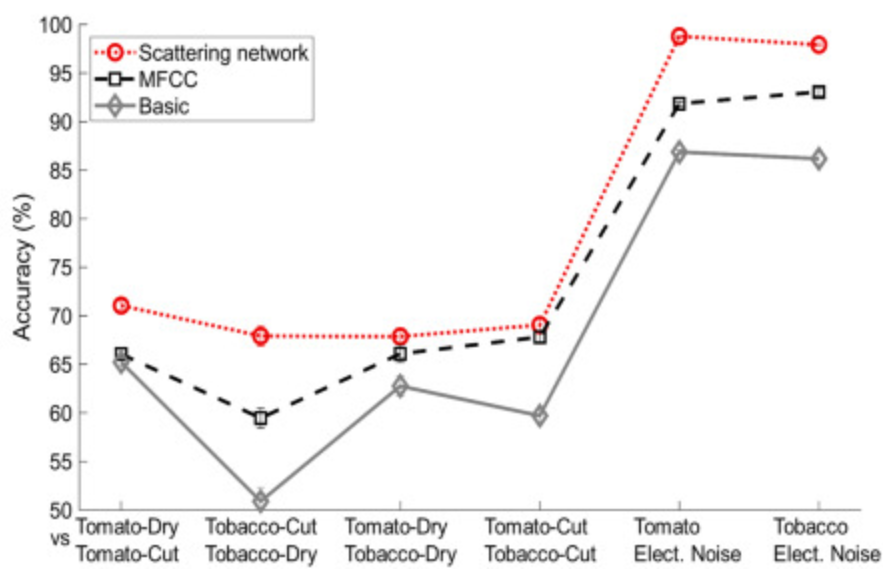
\includegraphics[width=\textwidth]{images/svm_classifier_results.png} % Adjust the image name and width as needed
    \caption{"The accuracy of sound classification achieved by different feature extraction methods, with an SVM classifier. The best results were obtained using the scattering network method for feature extraction (red). Using MFCC (black) for feature extraction the results were also highly significant and even basic methods (gray) for feature extraction allowed for better-than-random classification pair apart from one case: Tobacco dry vs. Tobacco cut, which was not significant with the basic method). The comparisons Tomato vs Elect. Noise and Tobacco vs Elect. Noise refer to electrical noise of the recording system." \cite{Cell_Sounds_emitted_by_plants}}
    \label{fig:image1}
  \end{subfigure}
  \hfill % Optional space between images
  \begin{subfigure}[b]{0.45\textwidth} % Adjust the width as needed
    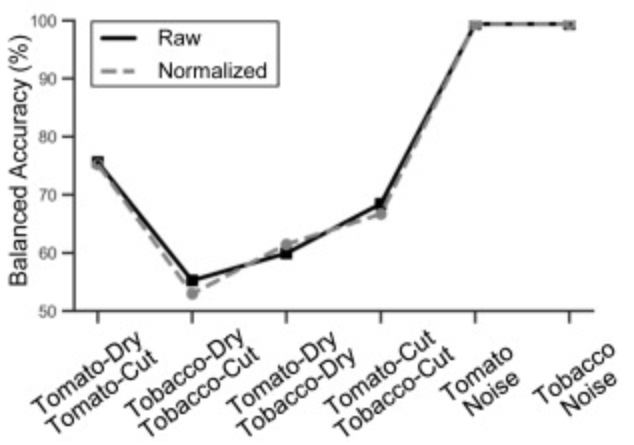
\includegraphics[width=\textwidth]{images/cnn_classifier_results.png} % Adjust the image name and width as needed
    \caption{"The accuracy of sound classification achieved by CNN models. The balanced accuracy of sound classification achieved by binary CNN models, for training and testing on the raw sound-vectors (black) and for training and testing on sound-vectors that were normalized by dividing each value in a vector by the vector’s maximal absolute value. Each balanced accuracy result is based on leave-one-plant-out cross validation." \cite{Cell_Sounds_emitted_by_plants}}
    \label{fig:image2}
  \end{subfigure}
  \caption{Comparison between SVM and CNN classifying plant stress type}
  \label{fig:images}
\end{figure}

\subsubsection{Leave-One-Plant-Out Cross-Validation (LOPO-CV)}
The Leave-One-Plant-Out Cross-Validation method was used to cross-validate the classification models. By treating every plant’s sound as a separate test set, this procedure makes the evaluation robust enough to withstand inter-plant variation bias within the samples. This approach serves more than one purpose: on the one hand it enhances generalizability; on the other hand, it provides direct proof that such models can work in real life situations involving variations from plant to plant.\cite{Cell_Sounds_emitted_by_plants}

\subsection{Overfitting}
One of the most problematic issue for CNN's and deep learning parctices in general is overfitting, meaning the model learns the training data too perfectly with all its details to the detriment of its performance in new, not seen data. Overfitting leads to losing the ability of the model to generalize well, hence rendering poor predictions on data not seen before.

In essence, overfitting means that the model is capturing noise or random fluctuations in the training data, instead of the underlying pattern that it is meant to learn. This occurs when a model is too complex, with too many parameters relative to the amount of training data. A very complex model tries to make the training data fit very closely but fails utterly in generalizing the new data; in other words, a very accurate model on the training data, but loses its accuracy when dealing with new data.

Detection of overfitting can be done by the comparing the performance of the model on the training dataset to another test dataset. Overfitting would be a clear case if the training set accuracy was very high and the test set accuracy much lower. Splitting the provided initial data set to separate the training and test sub-samples would thus help in approximating the model's performance on new data, hence the existence of potential overfitting.
\subsection{Data Augmentation}
Data augmentation is a technique designed to enhance the performances of a machine learning model by introducing artificial diversity into the training dataset. This is through applying different transformations not varied in the meaning of data and, therefore, the augmented data will still be associated with the same labels. This can be particularly beneficial in such areas where it is either complex or expensive to gather a huge dataset that is diverse. \cite{salamon_deep_2017}

Data augmentation in sound classification happens in many different ways and forms, with a nod towards the special nature of audio data. Some important methods of audio data augmentation include the following:

\begin{itemize}
    \item \textbf{Time Stretching (TS):}
    involves a process that makes audio samples play slower or faster without altering pitch. This may be beneficial to the model in terms of an invariance to the duration changes of sound events, which is very important in detecting sounds that might have occurred at different speeds.\cite{salamon_deep_2017}

    \item \textbf{Pitch Shifting (PS):} 
    This technique perturbs the pitch of the audio sample without changing its duration. The variation in pitch is naturally occurring as usually it occurs in varying environments; sounds of the same nature can have slightly differing pitches. \cite{salamon_deep_2017}
    
    \item \textbf{Dynamic Range Compression (DRC):} 
    This is a technique used to reduce the level difference between the loud and quiet portions of an audio signal. This will condition the dynamic range to be in uniformity; hence, the model can work well on recordings with varying degrees of loudness and dynamic range using different sets of compression.\cite{salamon_deep_2017}
    
    \item \textbf{Background Noise (BG):} 
    This refers to the original audio samples mixed with various background noises, such as sounds from the street or the park. This helps make the model resistant to environmental noise. This is an important consideration given that the applications in real-world scenarios are such that contain the target sounds mostly mixed with irrelevant background sounds.\cite{salamon_deep_2017}
\end{itemize}
    
All of these augmentations are applied directly to the audio signal before conversion into a spectrogram or any other representation used for the training of the network. Parameters for each augmentation should be chosen carefully to preserve the original semantic meaning of the audio. Although these data augmentation techniques have often improved the robustness and accuracy of sound classifiation models in different use cases, there is no evidence to this time that the mentioned methods can yield to better results in ultrasonic sound classification emitted by plants.
\subsection{Sound feature extraction}
Numerical representations of sound waves form the basis for audio features that allow algorithms to process and analyze sound beyond human perception. It is, therefore, important to extract these features as they have a bearing on how accurate and efficient the sound classification systems turn out. For classification of ultrasonic sounds emitted by plants that can be very complex, it is important to identify a set of features that accurately represent its characteristics.


\subsubsection{Mel Frequency Cepstral Coefficients (MFCC's)}
Mel Frequency Cepstral Coefficients (MFCCs) is a feature commonly used in speech and audio processing. This section explains what MFCCs are, why they’re used, and how they’re calculated.

\paragraph{Theoretical background}
The human ear's cochlea vibrates at different spots depending on the incoming sounds’ frequencies. This vibration can be modeled as a filter bank with triangular filters starting from low frequencies and moving upwards logarithmically until the highest ones are reached (Mel scale). The concept behind this non-linear frequency scale lies on how lower frequencies seem more easily distinguishable than higher ones by human ears. \cite{casale_physiology_2024}

Mel-frequency cepstrum coefficients are representations of the power spectrum of a sound in short time intervals. The term “cepstrum” derives from reversing the first four letters of “spectrum.” While normal cepstral representations work fine for some applications, MFCC's are designed to mimic the human ear's response more closely than the linearly-spaced frequency bands in order to better mimic the human ear’s response. This mimicking behavior is especially necessary for tasks like speech recognition or music analysis as well as feature extraction from those parts of acoustic spectrum where some sounds like plants produce frequencies outside normal hearing ranges. \cite{noauthor_mel-frequency_2024}


\textbf{Computational Process} \cite{gupta_feature_2013, zater_feature_2022}

\begin{figure}
    \centering
    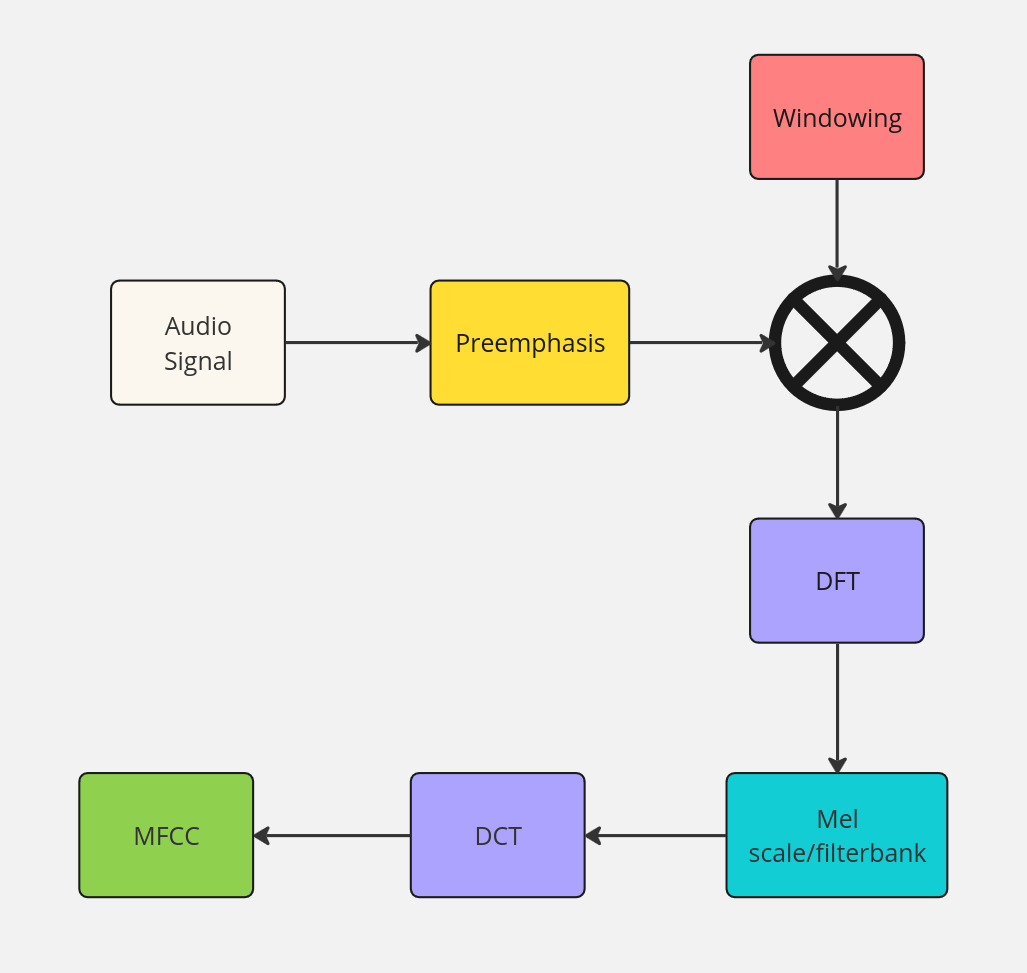
\includegraphics[width=0.5\linewidth]{images/mfcc_Flowchart.jpg}
    \caption{flowchart illustrating the fundamental process for computing Mel Frequency Cepstral Coefficients (MFCCs)}
    \label{fig:enter-label}
\end{figure}

\begin{enumerate}
    \item \textbf{Pre-emphasis:}
    The signal goes through an amplifyer to boost high frequencies in order to compensate for the decrease in magnitude at higher ones during recording.

    \item \textbf{Windowing:}
    The signal is sliced into short time frames. Windowing helps to minimize the signal discontinuities at the beginning and end of each frame. The window function, like a Hamming window, is typically applied to each frame to reduce the signal discontinuities at the boundaries.

    \item \textbf{DFT (Discrete Fourier Transform):}
    The Fourier Transform converts each frame of windowed signal from time domain to frequency domain, creating a spectrum for each frame.

    \item \textbf{Mel Filterbank:}
    Power spectrogram obtained from the DFT are then passed through a set of filters that simulates the non-linear human ear perception of pitch. Triangular and evenly spaced on the Mel scale.

    \item \textbf{Discrete Cosine Transform (DCT):}
    Finally, the log Mel spectrum is converted back into time domain by Discrete Cosine Transform, resulting in a time-domain representation of frequency information for each frame as a vector.
\end{enumerate}



MFCCs are used in various audio processes and machine learning tasks, particularly in speech recognition systems. Their ability to capture key features of human speech and the ear’s response makes them useful for distinguishing linguistic content and speaker characteristics in sound signals. They’ve been applied for voice recognition, music genre classification, emotion detection, and many other instances where sound is involved. \cite{zater_feature_2022}

Their use to classify plant sounds, specifically ultrasonic emissions that result from plants being under stress, is a new path of research. Plants produce a range of sounds in response to environmental threats, some of which fall outside our hearing abilities, so MFCCs’ accuracy and flexibility would be ideal. Analyzing these ultrasonic emissions could give researchers an understanding of plant health and stress levels, opening new doors in farming monitoring and care. \cite{Cell_Sounds_emitted_by_plants}

\subsubsection{Deep Scattering Spectrum (DSS)}
The Deep Scattering Spectrum (DSS) technology \cite{anden_deep_2014}, developed by Joakim Andén and Stéphane Mallat, represents a groundbreaking advancement in the audio classification domain. It is based on a mathematical framework of scattering transforms that allows for extraction of stable and invariant features from complex audio signals in an efficient manner.

DSS works by using scattering transform which is an extension of Mel-frequency cepstral coefficients (MFCCs), whereby modulation spectrum coefficients are integrated through multiple orders. This process consists of cascaded operations of wavelet convolutions and modulus operators. While traditional Fourier-based analyses may not be able to handle deformations such as time warping common in audio signals, scattering transforms are stable to time deformations while their local translation invariance remains intact.\cite{anden_deep_2014}

The second-order scattering coefficients are the core of the DSS method. Their job includes capturing transient events within audio; sudden attacks or amplitude modulations, which help distinguish complex sound patterns. The procedure starts with an initial wavelet transform followed by a modulus operation to obtain envelope information without losing energy over scales. Subsequent layers consist of wavelet transformations and modulus operations that reveal higher order features containing rich temporal and spectral information.\cite{anden_deep_2014}

DSS finds application within several realms of audio signal processing. DSS outperforms classical MFCC based techniques when it comes to musical genre classification since it captures wide range of audio characteristics leading to accurate identification of the genre. Due to its ability to identify subtle modulations and transient sounds even under noisy conditions, it is superior in classification for speech recognition purposes. An additional example can be seen in environmental sound analysis where distinguishing between complicated soundscapes is accomplished with ease by DSS. Ecosystem monitoring or urban sound classification would benefit from this sort of differentiation used for complex soundscapes. \cite{anden_deep_2014}

The study on ultrasonic sounds emitted by tomato and tobacco plants \cite{Cell_Sounds_emitted_by_plants} subjected to drought stress and physical injury were recorded and analyzed. It was possible for machine learning models trained using the scattering network features for differentiating between stressed and non-stressed plants thereby demonstrating that this method works in real life situations. Furthermore, this approach is also able not only to detect plant stress but also determine what kind of stress like dehydration or tissue damage.








% KONZEPT
%!TEX root=../main.tex
\chapter{Konzept}
Nach der Definition der Problemstellungen und Ziel soll recherchiert werden, wie diese erreicht, beziehungsweise gelöst werden können. Diese Studie beschäftigt sich mit möglichen Lösungen und Technologien und analysiert deren Eigenschaften um konkrete Vor- und Nachteile zu finden.
Beendet wird dieser Abschnitt mit einem Fazit.

Nachdem die Studie abgeschlossen und der Weg bestimmt ist soll nun ein Konzept oder eher noch ein Ablauf zur Lösung beschrieben werden. Hier finden sich Diagramme, Skizzen, Drehbücher, Mockups, ..., welche als Basis für die eigentliche Entwicklung verwendet werden.



% IMPLEMENTIERUNG
%!TEX root=../main.tex
\chapter{Implementierung}
Hier wird die Umsetzung des Projekts beschrieben und auf Details zu den einzelnen Technologien eingegangen. Im Optimalfall werden die Lösungen und Wege zu den zuvor definierten Problemen und Zielen geschildert. Eine bestehende Dokumentation, welche während der Arbeit erstellt wurde kann hier von großem Vorteil sein!

%!TEX root=../main.tex
\chapter{Retrospektive}
Kurz vor dem Ende wird der Verlauf des Projekts analysiert und geprüft, ob die Ziele erreicht und die Probleme gelöst wurden. Es wird auch auf Schwierigkeiten eingegangen, welche erst während der Arbeit zum Vorschein kamen und es können Verbesserungsvorschläge und Erkenntnisse vorgetragen werden.
Außerdem kann auch auf den weiteren Verlauf in der Zukunft eingegangen werden.
%!TEX root=../main.tex
\chapter{Conclusio} 
Hier findet eine letzte Zusammenfassung der Arbeit statt.
\include{chapters/Litaraturverzeichnis}

\begin{appendices}
\chapter{Calculation of microphone sensitivity}
\section{Understanding microphone sensitivity}
\end{appendices}

% \glsaddall	% Also list unused glossary entries
\end{document}
